\documentclass[tikz,border=2pt]{standalone}
\usepackage{tikz}
\usetikzlibrary{positioning}
\begin{document}
% Namikawa--Ueno type: IV^*-II_{l+1}
% Target MRNC type: IV^*_l
% Adapted from Tim Dokchitser picture: IV^*_{{\it n}}
% Parameter substitution: n -> l
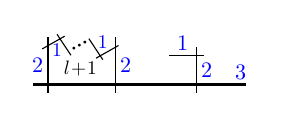
\begin{tikzpicture}[xscale=0.57,yscale=0.62]
\draw[thick,shorten >=2] (-1/3,0)--(68/15,0) node[inner sep=2pt,blue,above left,scale=0.8] {3};
\draw[shorten <=-3pt, shorten >=-3pt] (0,0)--node[inner sep=2pt,scale=0.8,blue,left] {2} (0,4/5);
\draw (0,4/5) 
    ++(-0.13,-0.07)--++(0.5,0.26)++(-0.19,-0.12)  
    ++(0.02,0)
      node[blue,scale=0.7,inner sep=1,anchor=north]{1}
    ++(-0.02,0)
    ++(0.02,0.16)--++(0.31,-0.43)++(0.07,0.13)  
    node{$\cdot$} ++(0.12,0.06) node{$\cdot$}
    ++(0.12,0.06) node{$\cdot$}++(-0.1,-0.17)    node[auto,inner sep=5,scale=0.7,anchor=north]{$l\!+\!1$}
    ++(0.19,0.26)--++(0.31,-0.43)++(0.04,0.18)   
    ++(-0.04,0)
      node[blue,scale=0.7,inner sep=1,anchor=south]{1}
    ++(0.04,0)
    ++(-0.04,-0.18)++(-0.15,0.03)--++(0.5,0.26);
\draw[shorten <=-3pt, shorten >=-3pt] (3/2,0)--node[inner sep=2pt,scale=0.8,blue,right] {2} (3/2,4/5);
\draw[shorten <=-3pt, shorten >=-3pt] (33/10,0)--node[inner sep=2pt,scale=0.8,blue,right] {2} (33/10,3/5);
\draw[shorten <=-3pt] (33/10,3/5)--node[inner sep=2pt,scale=0.8,blue,above] {1} (27/10,3/5);
\end{tikzpicture}
\end{document}
